\scanpage{33}
\mspage{4}

en l'ens. des nbs premiers qui sont distincts des caractéristiques résiduelles qui interviennent, vu que ce n'est que dans ce contexte modifié que l'on peut prouver des théorèmes qu'il faut \deleted{de trivialité}, cf Artin-Mazur ...).

On aura en particulier une suite exacte d'homotopie \deleted{\unsure{longue}} (choisissant un \deleted{``\unsure{pt base}''} ``pt base'' dans une série convenable \deleted{\unsure{p}} des germes d'espace $\mathcal V^*_{z,Z}$) :

\diagram{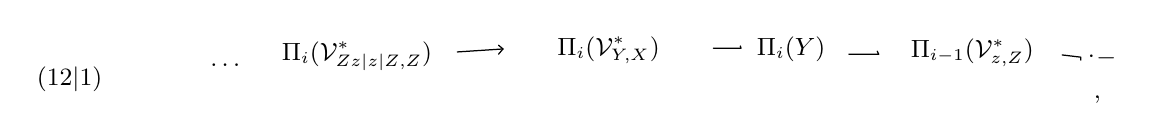
\begin{tikzpicture}[x=0.0095cm,y=-0.0095cm,font=\small,line width=0.45pt,line cap=round,line join=round]
\node at (42,105) {$(1\unsure{2|1})$};
\node at (250,86) {$\ldots$};
\node at (426,75) {$\Pi_i(\mathcal V^*_{\unsure{\deleted{Z}z|z|Z},Z})$};
\node at (762,67) {$\Pi_i(\mathcal V^*_{Y,X})$};
\node at (1006,66) {$\Pi_i(Y)$};
\node at (1248,70) {$\Pi_{i-1}(\mathcal V^*_{z,Z})$};
% The first connector has two wings; the next two have only short terminal returns.
\draw (560,69) -- (621,65);
\draw (615,60) -- (621,65) -- (615,72);
\draw (902,64) -- (939,64) -- (938,61);
\draw (1083,72) -- (1123,72) -- (1121,68);
% The terminal shaft and the visible clipped ellipsis fragment are not completed past the scan.
\draw (1368,73) -- (1393,76) -- (1393,80);
\node at (1407,75) {$\cdot$};
\node at (1427,78) {$-$};
\node at (1415,132) {,};
\end{tikzpicture}}

qui nous intéresse surtout en basses dimensions

\diagram{\begin{tikzpicture}[x=0.0095cm,y=-0.0095cm,font=\small,line width=0.45pt,line cap=round,line join=round]
\node at (48,100) {$(13)$};
\node at (295,88) {$\Pi_2(Y)$};
\node at (505,82) {$\Pi_1(\mathcal V^*_{z,Z})$};
\node at (796,68) {$\Pi_1(\mathcal V^*_{Y,X})$};
\node at (1059,78) {$\Pi_1(Y)$};
\node at (1288,75) {$\Pi_0(\mathcal V^*_{z,Z})$};
\node at (1296,264) {$\Pi_0(\mathcal V^*_{Y,X})$};
\node at (1278,422) {$\Pi_0(Y)$};
% Two incomplete rightward terminals, then two complete rightward heads.
\draw (366,83) -- (409,78) -- (405,75);
\draw (609,78) -- (670,77) -- (669,72);
\draw (920,77) -- (978,77);
\draw (971,70) -- (978,77) -- (971,84);
\draw (1146,74) -- (1193,74);
\draw (1188,69) -- (1193,74) -- (1188,79);
% Both downward shafts have visible terminal heads.
\draw (1265,130) -- (1269,207);
\draw (1262,200) -- (1269,207) -- (1274,201);
\draw (1281,312) -- (1284,374);
\draw (1279,369) -- (1284,374) -- (1288,369);
\node at (913,140) {$\underbrace{\hspace{3.83cm}}$};
% Additional small pen loop over the left part of the brace.
\draw (735,147) .. controls (754,133) and (778,132) .. (785,148);
\node at (928,192) {qui intervient dans $(10)$};
\end{tikzpicture}}

Si on suppose p. ex. que $z$ ne disconnecte pas $Z$ localement i.e. : \deleted{\unsure{donc}} la ``fibre $\mathcal V^*_{z,Z}$ est conne\unsure{x}
% The final cluster of the preceding word meets the paper/scan edge.
(ou encore, que $Y$ ne disconnecte pas $X$ loc\textsuperscript{t}.), alors $\Pi_1(\mathcal V^*_{Y,X})$ est une \uline{extension} de $\Pi_1(Y)$ par un quotient de $\Pi_1(\mathcal V^*_{z,Z})$, \deleted{\unsure{et}}

\margin{32}
